%=========================================================
% Memory Model 
%=========================================================
\section{Memory Model}

Memory Model of mmRISC-1 is based on the Little Endian order as shown in Figure \ref{fig:MEMORYMODEL}. As for instruction, both 16bit width code and 32bit width code should be aligned to 2-byte boundary. 32bit width code does not require its alignment to 4-byte boundary even if RV32C is not enabled.\\\\
As for data, 16bit data should be aligned to 2-byte boundary, and 32bit data should be aligned to 4- byte boundary. Unaligned data access invokes a memory alignment exception.\\\\
The mmRISC-1 uses strong memory access ordering. The sequence and the number of memory accesses are matched to the corresponding sequence of instructions executed. FENCE instruction is executed as NOP, FENCE.I instruction flushes the instruction fetch queue.

\begin{figure}[H]
    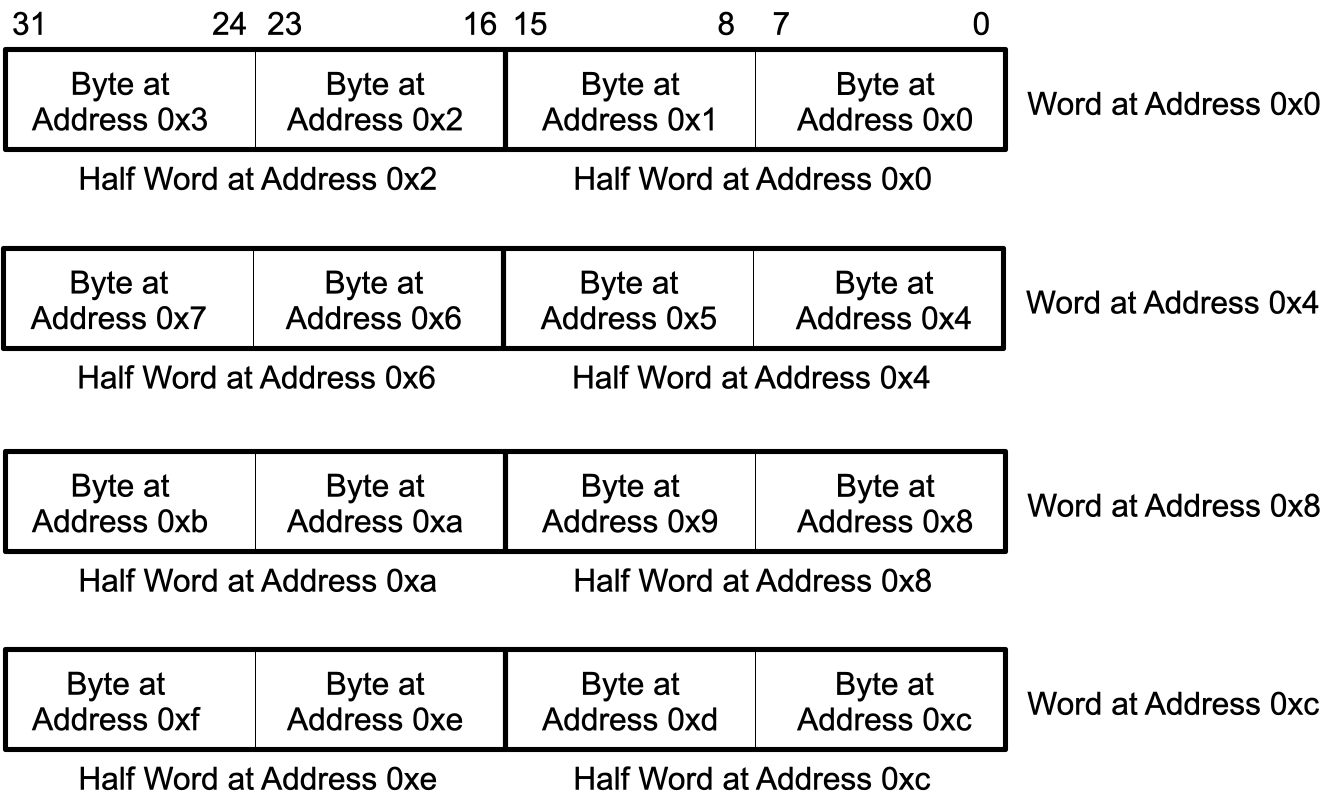
\includegraphics[width=1.00\columnwidth]{./Figure/MemoryModel.png}
    \caption{Little Endian Memory Organization}
    \label{fig:MEMORYMODEL}
\end{figure}



